% Options for packages loaded elsewhere
\PassOptionsToPackage{unicode}{hyperref}
\PassOptionsToPackage{hyphens}{url}
%
\documentclass[
  man]{apa6}
\usepackage{amsmath,amssymb}
\usepackage{iftex}
\ifPDFTeX
  \usepackage[T1]{fontenc}
  \usepackage[utf8]{inputenc}
  \usepackage{textcomp} % provide euro and other symbols
\else % if luatex or xetex
  \usepackage{unicode-math} % this also loads fontspec
  \defaultfontfeatures{Scale=MatchLowercase}
  \defaultfontfeatures[\rmfamily]{Ligatures=TeX,Scale=1}
\fi
\usepackage{lmodern}
\ifPDFTeX\else
  % xetex/luatex font selection
\fi
% Use upquote if available, for straight quotes in verbatim environments
\IfFileExists{upquote.sty}{\usepackage{upquote}}{}
\IfFileExists{microtype.sty}{% use microtype if available
  \usepackage[]{microtype}
  \UseMicrotypeSet[protrusion]{basicmath} % disable protrusion for tt fonts
}{}
\makeatletter
\@ifundefined{KOMAClassName}{% if non-KOMA class
  \IfFileExists{parskip.sty}{%
    \usepackage{parskip}
  }{% else
    \setlength{\parindent}{0pt}
    \setlength{\parskip}{6pt plus 2pt minus 1pt}}
}{% if KOMA class
  \KOMAoptions{parskip=half}}
\makeatother
\usepackage{xcolor}
\usepackage{graphicx}
\makeatletter
\def\maxwidth{\ifdim\Gin@nat@width>\linewidth\linewidth\else\Gin@nat@width\fi}
\def\maxheight{\ifdim\Gin@nat@height>\textheight\textheight\else\Gin@nat@height\fi}
\makeatother
% Scale images if necessary, so that they will not overflow the page
% margins by default, and it is still possible to overwrite the defaults
% using explicit options in \includegraphics[width, height, ...]{}
\setkeys{Gin}{width=\maxwidth,height=\maxheight,keepaspectratio}
% Set default figure placement to htbp
\makeatletter
\def\fps@figure{htbp}
\makeatother
\setlength{\emergencystretch}{3em} % prevent overfull lines
\providecommand{\tightlist}{%
  \setlength{\itemsep}{0pt}\setlength{\parskip}{0pt}}
\setcounter{secnumdepth}{-\maxdimen} % remove section numbering
% Make \paragraph and \subparagraph free-standing
\ifx\paragraph\undefined\else
  \let\oldparagraph\paragraph
  \renewcommand{\paragraph}[1]{\oldparagraph{#1}\mbox{}}
\fi
\ifx\subparagraph\undefined\else
  \let\oldsubparagraph\subparagraph
  \renewcommand{\subparagraph}[1]{\oldsubparagraph{#1}\mbox{}}
\fi
\newlength{\cslhangindent}
\setlength{\cslhangindent}{1.5em}
\newlength{\csllabelwidth}
\setlength{\csllabelwidth}{3em}
\newlength{\cslentryspacingunit} % times entry-spacing
\setlength{\cslentryspacingunit}{\parskip}
\newenvironment{CSLReferences}[2] % #1 hanging-ident, #2 entry spacing
 {% don't indent paragraphs
  \setlength{\parindent}{0pt}
  % turn on hanging indent if param 1 is 1
  \ifodd #1
  \let\oldpar\par
  \def\par{\hangindent=\cslhangindent\oldpar}
  \fi
  % set entry spacing
  \setlength{\parskip}{#2\cslentryspacingunit}
 }%
 {}
\usepackage{calc}
\newcommand{\CSLBlock}[1]{#1\hfill\break}
\newcommand{\CSLLeftMargin}[1]{\parbox[t]{\csllabelwidth}{#1}}
\newcommand{\CSLRightInline}[1]{\parbox[t]{\linewidth - \csllabelwidth}{#1}\break}
\newcommand{\CSLIndent}[1]{\hspace{\cslhangindent}#1}
\ifLuaTeX
\usepackage[bidi=basic]{babel}
\else
\usepackage[bidi=default]{babel}
\fi
\babelprovide[main,import]{english}
% get rid of language-specific shorthands (see #6817):
\let\LanguageShortHands\languageshorthands
\def\languageshorthands#1{}
% Manuscript styling
\usepackage{upgreek}
\captionsetup{font=singlespacing,justification=justified}

% Table formatting
\usepackage{longtable}
\usepackage{lscape}
% \usepackage[counterclockwise]{rotating}   % Landscape page setup for large tables
\usepackage{multirow}		% Table styling
\usepackage{tabularx}		% Control Column width
\usepackage[flushleft]{threeparttable}	% Allows for three part tables with a specified notes section
\usepackage{threeparttablex}            % Lets threeparttable work with longtable

% Create new environments so endfloat can handle them
% \newenvironment{ltable}
%   {\begin{landscape}\centering\begin{threeparttable}}
%   {\end{threeparttable}\end{landscape}}
\newenvironment{lltable}{\begin{landscape}\centering\begin{ThreePartTable}}{\end{ThreePartTable}\end{landscape}}

% Enables adjusting longtable caption width to table width
% Solution found at http://golatex.de/longtable-mit-caption-so-breit-wie-die-tabelle-t15767.html
\makeatletter
\newcommand\LastLTentrywidth{1em}
\newlength\longtablewidth
\setlength{\longtablewidth}{1in}
\newcommand{\getlongtablewidth}{\begingroup \ifcsname LT@\roman{LT@tables}\endcsname \global\longtablewidth=0pt \renewcommand{\LT@entry}[2]{\global\advance\longtablewidth by ##2\relax\gdef\LastLTentrywidth{##2}}\@nameuse{LT@\roman{LT@tables}} \fi \endgroup}

% \setlength{\parindent}{0.5in}
% \setlength{\parskip}{0pt plus 0pt minus 0pt}

% Overwrite redefinition of paragraph and subparagraph by the default LaTeX template
% See https://github.com/crsh/papaja/issues/292
\makeatletter
\renewcommand{\paragraph}{\@startsection{paragraph}{4}{\parindent}%
  {0\baselineskip \@plus 0.2ex \@minus 0.2ex}%
  {-1em}%
  {\normalfont\normalsize\bfseries\itshape\typesectitle}}

\renewcommand{\subparagraph}[1]{\@startsection{subparagraph}{5}{1em}%
  {0\baselineskip \@plus 0.2ex \@minus 0.2ex}%
  {-\z@\relax}%
  {\normalfont\normalsize\itshape\hspace{\parindent}{#1}\textit{\addperi}}{\relax}}
\makeatother

% \usepackage{etoolbox}
\makeatletter
\patchcmd{\HyOrg@maketitle}
  {\section{\normalfont\normalsize\abstractname}}
  {\section*{\normalfont\normalsize\abstractname}}
  {}{\typeout{Failed to patch abstract.}}
\patchcmd{\HyOrg@maketitle}
  {\section{\protect\normalfont{\@title}}}
  {\section*{\protect\normalfont{\@title}}}
  {}{\typeout{Failed to patch title.}}
\makeatother

\usepackage{xpatch}
\makeatletter
\xapptocmd\appendix
  {\xapptocmd\section
    {\addcontentsline{toc}{section}{\appendixname\ifoneappendix\else~\theappendix\fi\\: #1}}
    {}{\InnerPatchFailed}%
  }
{}{\PatchFailed}
\DeclareDelayedFloatFlavor{ThreePartTable}{table}
\DeclareDelayedFloatFlavor{lltable}{table}
\DeclareDelayedFloatFlavor*{longtable}{table}
\makeatletter
\renewcommand{\efloat@iwrite}[1]{\immediate\expandafter\protected@write\csname efloat@post#1\endcsname{}}
\makeatother
\usepackage{csquotes}
\ifLuaTeX
  \usepackage{selnolig}  % disable illegal ligatures
\fi
\IfFileExists{bookmark.sty}{\usepackage{bookmark}}{\usepackage{hyperref}}
\IfFileExists{xurl.sty}{\usepackage{xurl}}{} % add URL line breaks if available
\urlstyle{same}
\hypersetup{
  pdftitle={Demanding resources: Converging perceptions of challenge and resource characteristics},
  pdfauthor={John Kulas1, Alicia Stachowski2, \& Renata García Prieto Palacios Roji3},
  pdflang={en-EN},
  hidelinks,
  pdfcreator={LaTeX via pandoc}}

\title{Demanding resources: Converging perceptions of challenge and resource characteristics}
\author{John Kulas\textsuperscript{1}, Alicia Stachowski\textsuperscript{2}, \& Renata García Prieto Palacios Roji\textsuperscript{3}}
\date{}


\shorttitle{Demanding Resources}

\authornote{

Correspondence concerning this article should be addressed to John Kulas. E-mail: \href{mailto:jtkulas@ergreports.com}{\nolinkurl{jtkulas@ergreports.com}}

}

\affiliation{\vspace{0.5cm}\textsuperscript{1} eRg\\\textsuperscript{2} University of Wisconsin - Stout\\\textsuperscript{3} PepsiCo}

\abstract{%
Using the Challenge-Hindrance Framework, 2 research questions were examined: are jobs with many resources also perceived to have many challenges, and 2) could that association be moderated by kind of job characteristic. A survey of 568 workers rated job characteristics in terms of relevance as well as perceptions as challenges, hindrances and resources using the common O*NET classification of work activities and context.The findings point to high association between the number of resources and challenge demands employees experience, reasonable correspondence or agreement that a characteristic is a resource \emph{and} challenge, and differences in this association by job characteristic category. More variability was observed when exploring associations between resources and hindrance stressors, and challenge/hindrance stressors.
}



\begin{document}
\maketitle

The Occupational Information Network (O*NET; onetonline.org) contains a reasonably comprehensive description of occupations (Peterson et al., 2001) which subject matter experts inform via surveys. In the current study, we utilize a set of O*NET job context and activity statements to explore two questions about how people perceive resources, challenges, and hindrances within their jobs. \footnote{There are a number of advantage to using this standard set of statements, but the primary one here lies in our ability to consider a wide range of job characteristics, with a focus on individual perceptions of each rather than limiting ourselves to a more generic set of demands or those of a limited scope.} Here, we focus broadly on two research questions using these O*NET items: 1) are jobs with many resources also perceived to have many challenges, and 2) could that association be moderated by kind of job characteristic (e.g., interacting with others vs.~physical work characteristics)? The basis for these questions comes out the stress literature (e.g., Lazarus \& Folkman, 1984).

We argue below that \emph{perception} of something as a resource or demand matters. Although the word ``stress'' often carries a negative connotation, the ``father'' of the current concept, Selye (1936), conceptualized stress much less pejoratively - rather thinking of it as a \emph{response to change}. For instance, consider the different reactions two different employees may have to being nominated to give a speech at an upcoming company event. One may appraise the nomination as a negative stressor. However, another employee may appraise the nomination to do so as an opportunity to share their experiences with more of their coworkers, or one in which they may receive recognition they have desired. Selye the physician would likely have labeled the two responses as subjective manifestations of ``distress'', and ``eustress'' (Selye, 1974).

\hypertarget{not-all-stressors-are-equal-the-challenge-hindrance-framework}{%
\subsection{Not all Stressors are Equal: The Challenge-hindrance Framework}\label{not-all-stressors-are-equal-the-challenge-hindrance-framework}}

In modern I-O psychology parlance (and more consistent with the job demands-resources model (Demerouti et al., 2001) and job demands-resources theory (Bakker \& Demerouti, 2017)), the two workers above would both be characterized as appraising the speaking opportunity as a job demand. However, as noted above, demands/stressors are subjective. Cavanaugh's (2000) challenge-hindrance stressor framework speaks directly to this reality, and suggests that the way we understand reactions to stressors requires consideration of how people \emph{feel} about a given stressor. One of our above employees would be appraising the demand as a \emph{challenge} while the other would appraise the demand as a \emph{hindrance} (Cavanaugh et al., 2000). According to Cavanaugh et al. (2000), challenge demands promote mastery, personal growth, and future gains. Challenge stressors should lead to coping strategies that facilitate achievement and motivation (e.g., Kim \& Beehr, 2020). Hindrance demands, in contrast, inhibit growth, learning and goal achievement (e.g., perception of role conflict, workplace politics). Perhaps not surprisingly, challenge demands are typically associated with positive outcomes, whereas hindrance demands are associated with more negative outcomes (e.g., Cavanaugh et al., 2000).

LePine (2022) explain the mechanisms by which demands are related to these differential positive and negative outcomes. Similar to the job-demands resources theory (Bakker \& Demerouti, 2017), challenge and hindrance demands elicit two different paths or processes. Challenge stressors typically result in a challenge appraisal, and engagement is likely to happen as a result. Engagement is positively related to the positive outcomes described above: motivation, performance, growth, and wellbeing. Of note is that this energy may be depleted eventually, leading to strain. Rosen et al. (2020), in fact, suggests that appraisals may change over time, which is probably expected when thinking about how workers experience continued stressors. Hindrance stressors elicit a different process. Rather than experiencing engagemnet, disengagement is likely to result from a hindrance appraisal, which in contrast, negatively impacts motivation, performance, growth and wellbeing. This is a result of depleted resources via frustrations and other affectively negative reactions (LePine, 2022).

Recently, Horan et al. (2020) and LePine (2022) have both called out the need for additional research to incorporate the \emph{appraisal process} described by Lazarus and Folkman (1984) into the challenge-hindrance stressor framework, which aligns with other calls to capture subjective ratings of demands and resources into our study of the overarching job demands-resources model. In fact, Horan et al. (2020) state that ``\ldots stressors are only challenge or hindrance stressors to the extent that they are perceived as such by employees'' (p.~3). In the current study, we build on the work of a growing number of researchers who argue that the characteristics of work may be appraised simultaneously as resources \emph{and} demands (Webster et al., 2011).

\hypertarget{current-study-and-research-questions}{%
\subsection{Current Study and Research Questions}\label{current-study-and-research-questions}}

At the most broad level, we can question whether employees actually distinguish between challenges and hindrances as the theory describes. Research suggests that people can and do perceive them differently. For example, Bakker and Sanz-Vergel (2013) found that perceived work pressure can be classified as a hindrance demand, while the requirement to express emotions is a challenge demand. Webster et al. (2011) also considered three common work characteristics including workload, role ambiguity, and role conflict. Interestingly, they found that while each could be identified \emph{primarily} as a challenge or hindrance, employees could also appraise that a characteristic is simultaneously both a challenge and hindrance. However, this list of demands (workload, role ambiguity, and role conflict) is somewhat narrow. Using a very wide range of O*NET job characteristics regarding job context and activities, we explore whether challenges (positive stressors per the definition above) might actually be positively related to resources. Per the job demands-resources theory (Bakker \& Demerouti, 2017) resources are defined as physical, psychological, social, or organizational aspects of the job that may help an employee achieve work goals, reduce job demands, or promote personal growth and development (Demerouti et al., 2001). It stands to reason that a challenging demand may be considered a resource.

\emph{RQ1}: Do employees who perceive many resources in their jobs also perceived many challenges?

Although we argue that the same job characteristic may be perceived as both a challenge and a resource, it is also likely that some characteristics are less likely to be viewed as mutually complementary as others. For example, a physically strenuous job requirement such as ``carrying heavy objects'' would be less likely to be viewed both as a challenge and a resource whereas a structural characteristic such as ``negotiating work schedules'' may very well be viewed (likely in different circumstances) to be both a control-oriented resource as well as a challenge. O*NET has different levels of abstraction with regard to the nature of job characteristics. We will be exploring a mid-level abstraction with seven different characteristic scales.

\emph{RQ2}: Is the association between resource and challenge characteristics moderated by type of characteristic?

\hypertarget{method}{%
\section{Method}\label{method}}

We evaluate agreement across perceptions of job characteristics regarding their characterization as resource, challenge, and hindrance (Bakker \& Demerouti, 2017; Bakker et al., 2003; Demerouti et al., 2001). To capture an effectively exhaustive list of characteristics that apply to, theoretically, \emph{every} possible job, we consult the unifying framework of O*NET.

\hypertarget{participants}{%
\subsection{Participants}\label{participants}}

Eligibility requirements included being 18 or older and holding either a full- or part-time job. Participants were asked to think about their primary job while answering the survey. We sampled from a Prolific panel, resulting in 785 individuals who initially accessed the survey link. Of those, 112 indicated that they were not interested, had more than 200 missing responses, or had 20 or more identical consecutive sequential responses (Yentes \& Wilhelm, 2021). Additional screening using four embedded attention checks resulted in the retention of 568 respondents. A total of 13.57\% had been in their job less than 6 months, 19.20\% between 6 months and a year, 49.12\% between one and five years, 13.27\% between 5 and 10 years, and 4.87\% more than 10 years. Reported ages ranged from 18 to 65 with an average of 28.18 years old (SD = 7.53). Gender was captured via a free-field gender identity category, although the sample predominantly self-identified as female (52.6\%) or male (46.8\%).

\hypertarget{materials}{%
\subsection{Materials}\label{materials}}

Our survey was informed by 98 statements taken from job characteristic descriptors located within O*NET's classification of ``work activities'': 1) Information Input (5 statements), 2) Interacting with Others (17 statements), 3) Mental Processes (10 statements), and 4) Work Output (9 statements) and ``work context'' groupings: 1) Interpersonal Relationships (14 statements), 2) Physical Work Conditions (30 statements), and 3) Structural Job Characteristics (13 statements).

The O*NET descriptors are written in a similar manner to a task statement presented within a job analysis, but the level of abstraction is closer to ``responsibility'' than task. For example, the descriptor for ``level of competition'', which is an element of the ``structural job characteristics'' grouping, is \emph{How often do you have to perform public speaking in this job??} Other than minor grammatical editing (for example, changing ``the worker'' to ``you'' where applicable), we retained the O*NET wording for our item stems. We also retained O*NET's response scales, several of which were semantically unique across items, but all shared the same 5-point scale. It would likely NOT be considered controversial to referred to these as ``effectively'' Likert-type response scales.

\hypertarget{procedure}{%
\subsection{Procedure}\label{procedure}}

Respondents were recruited through Prolific. After providing consent, respondents provided ratings of whether or not each of the 98 O*NET characteristics were relevant for the respondent's primary work role. Subsequently, each respondent who agreed that an element had at least some relevance to their job was then also asked to rate that element in terms of perception of resource, challenge, and hindrance. The total number of items on the survey was less than 392 (98 characteristics x 4 administrations - the first for relevance and the remaining 3 for resources, challenges, and hindrances) because we did not ask for demand and resource evaluations for 14 O*NET characteristics that we projected would have very low frequency of endorsement across respondents (one excluded characteristic, for example, was \emph{\ldots the extent to which the worker is exposed to radiation on the job}). Furthermore, not every respondent indicated that the same characteristics were relevant to them. Therefore, each respondent had a unique set of administered items. Participants were compensated for their participation in this study in the amount of six dollars through Prolific.

\hypertarget{results}{%
\section{Results}\label{results}}

All analyses are focused on characteristics of work that were rated as being ``relevant'' to the respondents' primary job. Upon confirming that a work characteristic was relevant, respondents then also rated the extent to which that characteristic was perceived as a resources, challenge, and hindrance.

\begin{table}[tbp]

\begin{center}
\begin{threeparttable}

\caption{\label{tab:cortab}Resource, challenge, and hindrance correlations (counts data).}

\begin{tabular}{lllll}
\toprule
 & \multicolumn{1}{c}{1} & \multicolumn{1}{c}{2} & \multicolumn{1}{c}{$M$} & \multicolumn{1}{c}{$SD$}\\
\midrule
1. resource & - &  & 36.02 & 13.26\\
2. hindrance & .23*** & - & 13.09 & 13.62\\
3. challenge & .86*** & .22*** & 35.64 & 13.63\\
\bottomrule
\end{tabular}

\end{threeparttable}
\end{center}

\end{table}

\begin{figure}
\centering
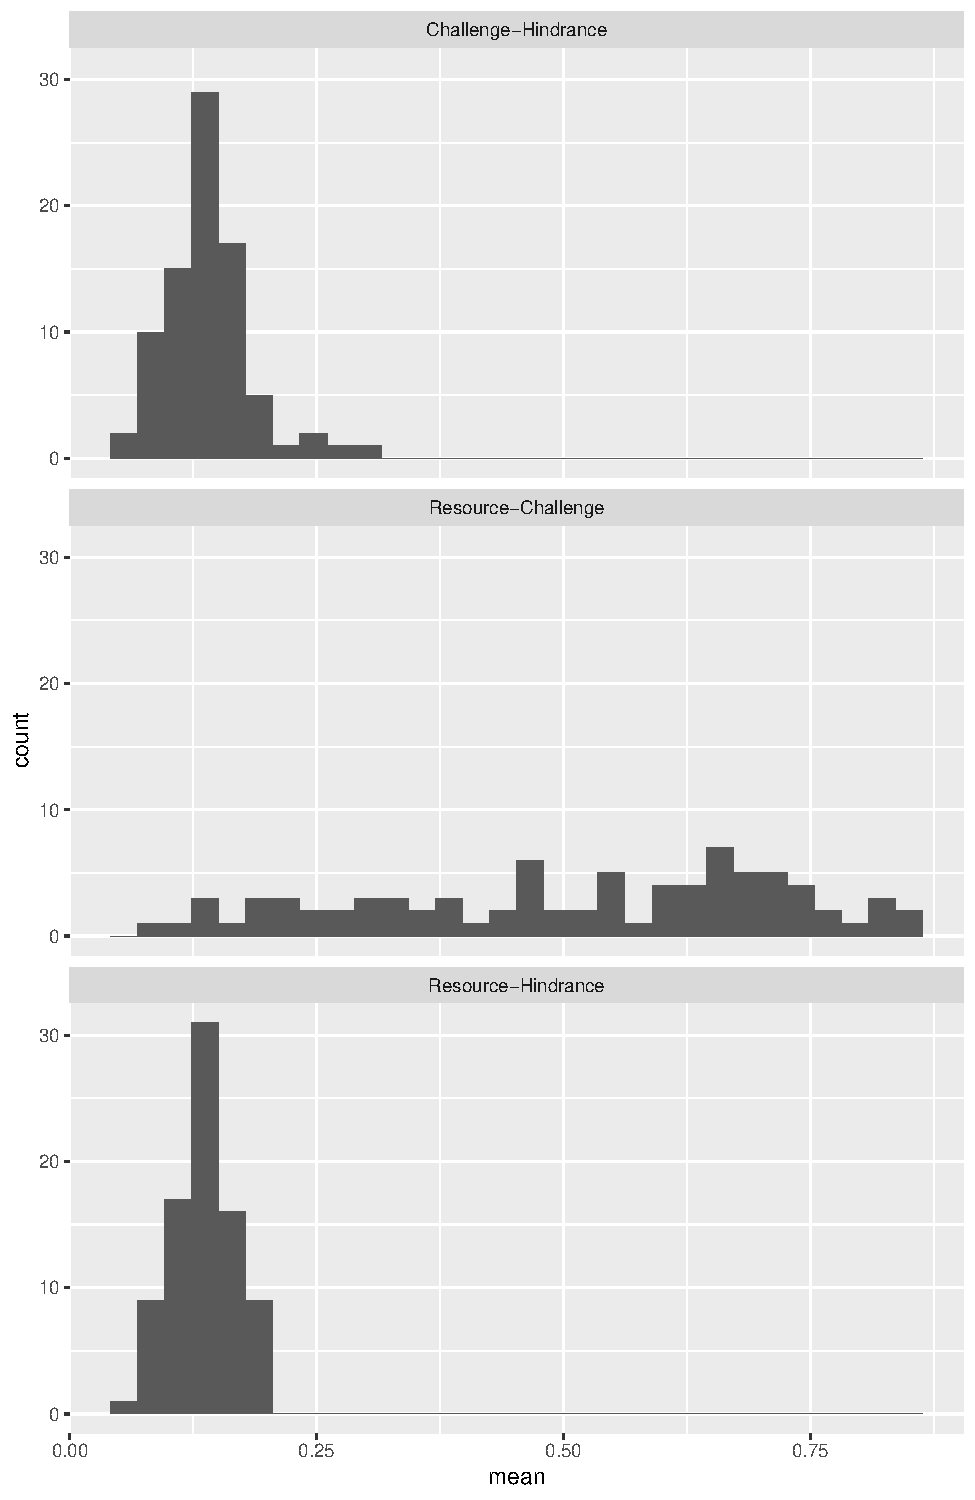
\includegraphics{SIOP2024convergence_files/figure-latex/percagree-1.pdf}
\caption{\label{fig:percagree}Percent convergence (characteristic rated consistently as, for example, both a resource and a hindrance).}
\end{figure}

\begin{figure}
\centering
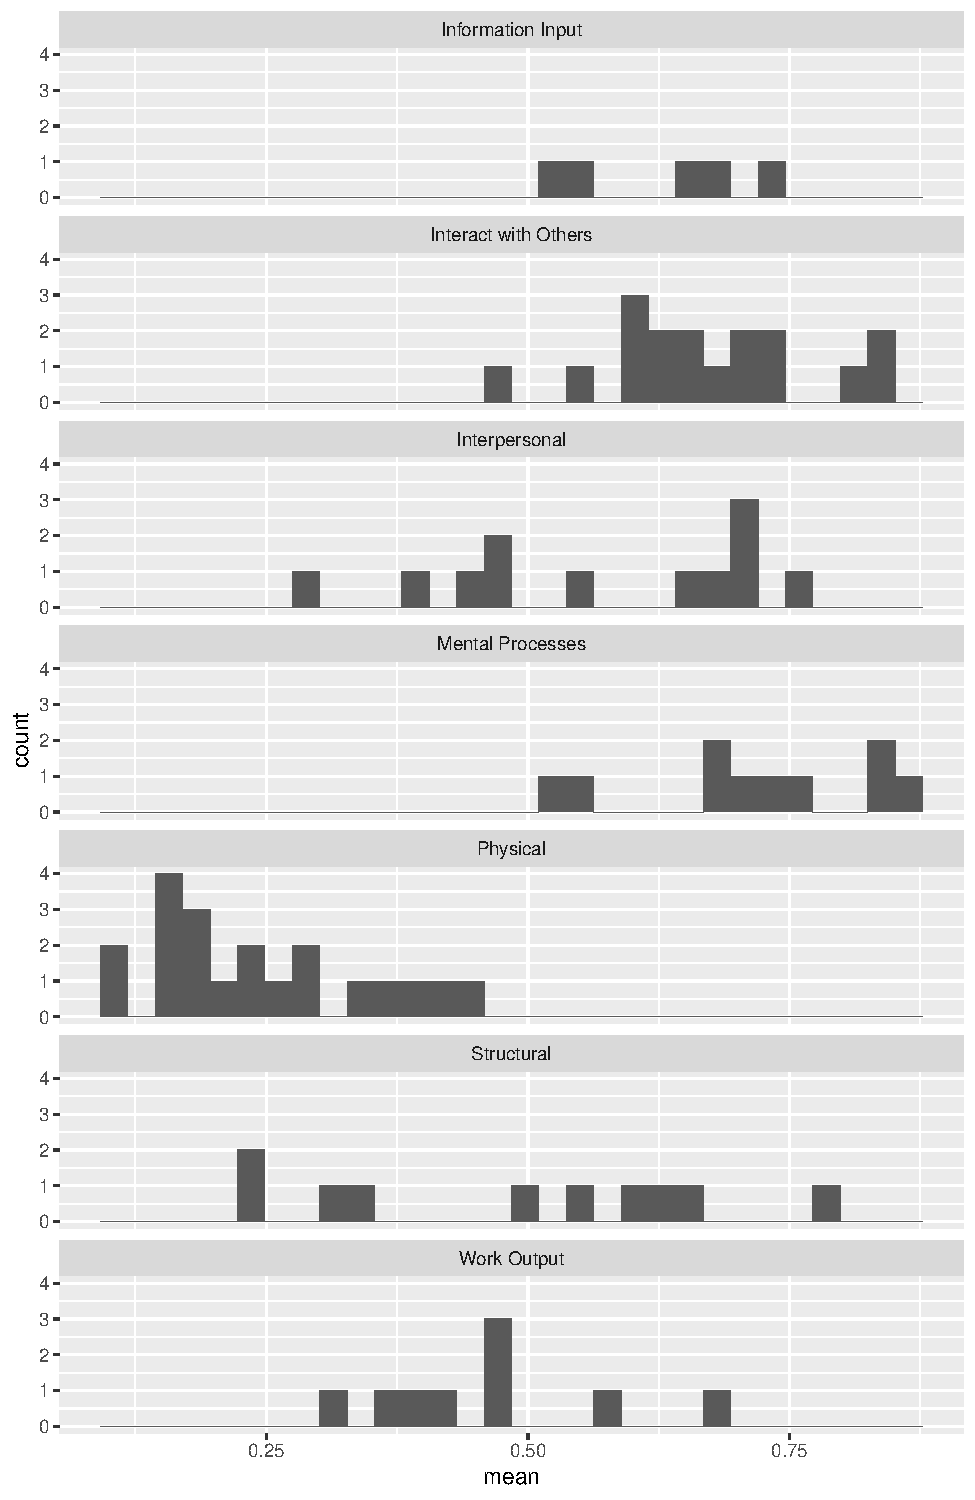
\includegraphics{SIOP2024convergence_files/figure-latex/recchall-1.pdf}
\caption{\label{fig:recchall}Resource and challenge agreement across ONet characteristic groupings (e.g., scales).}
\end{figure}

\hypertarget{resource-challenge-and-hindrance-associations}{%
\subsection{Resource, Challenge, and Hindrance Associations}\label{resource-challenge-and-hindrance-associations}}

Research Question 1 explored whether people who perceive many challenges in their work also report many resources. The results show that the total number of undifferentiated challenges and resources are positively related. In fact, table \ref{tab:cortab} shows a very high association between resources and challenges (\emph{r} = .86). This association, however, only captures the relationship between these demands and resources in \emph{sheer volume}. That is, Table \ref{tab:cortab} operationalized each variable as the sheer number of resources, hindrances, or challenges that a respondent indicated were present within their job. This correlational analysis \emph{does} imply that workers who experience more resources also perceive greater challenges. Although not explicitly part of the above research question, we also explored the associations between resources and hindrances (\emph{r} = .23) and challenges and hindrances (\emph{r} = .22), which were also significantly positive with moderate in magnitude, suggesting that some of this ``sheer volume'' may be capturing job complexity (that is, the more complex the job, the more characteristics are relevant, and therefore the more likely it is to have \emph{more} challenges as well as \emph{more} hindrances as well as \emph{more} resources). Although we did not address job complexity as a moderator in the current paper, we do plan to do so in future investigations. Also, take note of the average numbers of resources, challenges, and hindrances cited by our sample, where these respondents generally experienced fewer hindrances in their jobs (\emph{M} = 13.09) than both resources and challenges.

We further explored whether the mean number of resources, challenge- and hindrance demands were signficantly different from one another. Mirroring the results above, a paired-samples t-test between mean number of resources and challenges suggests that respondents did not experience more resources than challenges, \emph{t}(567), = 1.29, \emph{p} = .198, 95\% CI = {[}-0.20, 0.96{]}, \emph{d} = 0.03. However, there was a significant difference between mean number of resources and hindrances, suggesting respondents experienced more resources than hindrances, \emph{t}(567), = 32.67, \emph{p} \textless{} .001, 95\% CI = {[}21.55, 24.31{]}, \emph{d} = 1.71, and between mean number of challenges and hindrances suggests that respondents experienced more challenges than hindrances, \emph{t}(567), = -31.58, \emph{p} \textless{} .001, 95\% CI = {[}-23.95, -21.15{]}, \emph{d} = 1.65. In sum, these findings highlight a pattern in which those who perceive or experience challenges in their work also perceive more resources, the implications of which will be explored further in the discussion.

\hypertarget{correspondence-between-individual-job-characteristic-perceptions}{%
\subsection{Correspondence between Individual Job Characteristic Perceptions}\label{correspondence-between-individual-job-characteristic-perceptions}}

While interesting, we note above that the initial analyses explore this question through a very broad ``sheer volume'' lens. We next looked for convergence of perception at the level of each \emph{individual job characteristic}. Here, we calculated the \emph{percent of affirmative correspondence} between individual characteristic perceptions. That is, a respondent needed to agree that \emph{\ldots being in contact with others} was both a resource as well as a challenge in order to be implicated as affirmatively agreeing. We did this for each of the 84 individual characteristics that were rated as a resource, challenge, or demand and then computed an aggregate level of affirmative correspondence for each person. Figure \ref{fig:percagree} presents the results of these correspondences, showing that there was not much mutual agreement regarding characteristics being viewed as both hindrances and resources (\emph{M} = 0.14) or as challenges and hindrances (\emph{M} = 0.14). However, when a characteristic was viewed a resource, it was more likely to also be perceived as a challenge (although the correspondence also exhibited quite a bit of variability; \emph{M} = 0.51, \emph{SD} = 0.21).

\hypertarget{is-the-association-between-resource-and-challenge-characteristics-moderated-by-type-of-characteristic}{%
\subsection{Is the association between resource and challenge characteristics moderated by type of characteristic?}\label{is-the-association-between-resource-and-challenge-characteristics-moderated-by-type-of-characteristic}}

Figure \ref{fig:recchall} explores the possibility of moderation by \emph{type of characteristic rated} for the resource-challenge convergence (RQ2). Here, we categorized each characteristic by its O*NET ``scale'' (one of seven), and the graph shows greater consistency across certain characteristics (for example, \emph{Mental Processes} or \emph{Interacting with Others}) and less convergence across other \emph{types} of job activities (for example, \emph{Physical} characteristics). A repeated-measures ANOVA retaining these scales as 7 different levels of a within-subjects' independent variables yielded a treatment effect of \(F_{(6, 3,402)}\) = 613.5, \emph{p} \textless{} .001, \(\eta^2_{p}\) = 0.21 (the subjects' effect was \(F_{(567, 3402)}\) = 6.13, \emph{p} \textless{} .001). The only contrast not broaching statistical significance via Bonferonni-corrected pairwise t-tests was Work Output vs.~Structural job characteristics (\emph{t} = -1.10). The largest contrasts were Physical work conditions vs.~Structural job characteristics (\emph{t} = 25.14), Interpersonal relationships (\emph{t} = -29.25), Mental processes (\emph{t} = -33.84), and Interacting with others (\emph{t} = -35.60)

\hypertarget{discussion}{%
\section{Discussion}\label{discussion}}

The major goal of this paper was to further explore the relationships among perceptions of job characteristics as challenge demands, hindrance demands, and resources. Our findings suggest that there is an association between the number of resources and challenges employees perceive, and that this association does appear to be moderated by type of job characteristic. The results highlight the importance of dissociating the \emph{nature} of job demands, as we did not see the same patterns across challenge and hindrance demands.

Similar to the eustress/distress distinction (e.g., Selye, 1974), it would seem as though demands should perhaps be thought of in a valenced manner (e.g., is it a ``good'' demand or a ``bad'' demand). Distinguishing between different kinds of work demands has implications for not only the employees themselves, but also teams they may be a part of, managers and the like. This is because demands appraised as a challenge promote mastery, personal growth, and future gains. Moreover, it was more likely that employees would also perceive these characteristics as \emph{resources} within their jobs.

In terms of convergence of resource and challenge appraisals, there was quite a bit of variability (e.g., Figure \ref{fig:percagree}), but that variability was partially explained by the nature of the characteristic being evaluated (e.g., Figure \ref{fig:recchall}). Physical job characteristics such as, for example, the amount of ``time spent bending or twisting the body'' may be much more likely to be appraised as a challenging demand (but not a resource). Other \emph{types} of job requirements, however, such as a mental process like, ``scheduling work and activities'' might reasonably be expected to exhibit greater convergence. We suspect that there are other moderators that help explain this association/ disassociation between challenges and resources, and would like to incorporate variables such as a respondents' personality in future investigations.

\hypertarget{limitations-future-directions}{%
\subsection{Limitations \& Future Directions}\label{limitations-future-directions}}

The findings above point to a number of additional avenues for this line of research. While our study focused on activity and content O*NET statements, we were practically limited in the number of items that could be administered. As such, it would be of value to explore other, additional job characteristics, particularly in the relational realm (e.g., the ``human'' resources that are a major component of most work such as interacting with coworkers, one's relationship with a supervisor). Another important direction to consider will be that of job type. We explored one potential moderator - that of job characteristic category, but it is also quite possible that those in certain industries experience some job characteristics with more frequency and would naturally have more resources/challenges, for instance. Individual differences in person-job fit may also prove to be a useful addition, as would outcomes associated with resources and demands at work (e.g., job satisfaction, engagement, intent to turnover).

\hypertarget{conclusion}{%
\subsection{Conclusion}\label{conclusion}}

This study contributes to our understanding of the experience of different characteristics of work using the common O*NET classification of work activities and context. The findings point to high association between the number of resources and challenge demands employees experience, reasonable correspondence or agreement that a characteristic is a resource \emph{and} challenge, and differences in this association by job characteristic category. More variability was observed when exploring associations between resources and hindrance stressors, and challenge/hindrance stressors. The results speak strongly to the importance of perceptions of resources and demands at work given existing literature on the outcomes associated with such appraisals.

\hypertarget{references}{%
\section*{References}\label{references}}
\addcontentsline{toc}{section}{References}

\hypertarget{refs}{}
\begin{CSLReferences}{1}{0}
\leavevmode\vadjust pre{\hypertarget{ref-bakker2017job}{}}%
Bakker, A. B., \& Demerouti, E. (2017). Job demands--resources theory: Taking stock and looking forward. \emph{Journal of Occupational Health Psychology}, \emph{22}(3), 273.

\leavevmode\vadjust pre{\hypertarget{ref-bakker2013weekly}{}}%
Bakker, A. B., \& Sanz-Vergel, A. I. (2013). Weekly work engagement and flourishing: The role of hindrance and challenge job demands. \emph{Journal of Vocational Behavior}, \emph{83}(3), 397--409.

\leavevmode\vadjust pre{\hypertarget{ref-cavanaugh2000empirical}{}}%
Cavanaugh, M. A., Boswell, W. R., Roehling, M. V., \& Boudreau, J. W. (2000). An empirical examination of self-reported work stress among US managers. \emph{Journal of Applied Psychology}, \emph{85}(1), 65.

\leavevmode\vadjust pre{\hypertarget{ref-demerouti2001job}{}}%
Demerouti, E., Bakker, A. B., Nachreiner, F., \& Schaufeli, W. B. (2001). The job demands-resources model of burnout. \emph{Journal of Applied Psychology}, \emph{86}(3), 499.

\leavevmode\vadjust pre{\hypertarget{ref-horan2020review}{}}%
Horan, K. A., Nakahara, W. H., DiStaso, M. J., \& Jex, S. M. (2020). A review of the challenge-hindrance stress model: Recent advances, expanded paradigms, and recommendations for future research. \emph{Frontiers in Psychology}, \emph{11}, 560346.

\leavevmode\vadjust pre{\hypertarget{ref-kim2020thriving}{}}%
Kim, M., \& Beehr, T. A. (2020). Thriving on demand: Challenging work results in employee flourishing through appraisals and resources. \emph{International Journal of Stress Management}, \emph{27}(2), 111.

\leavevmode\vadjust pre{\hypertarget{ref-lazarus1984stress}{}}%
Lazarus, R. S., \& Folkman, S. (1984). \emph{Stress, appraisal, and coping}. Springer publishing company.

\leavevmode\vadjust pre{\hypertarget{ref-lepine2022challenge}{}}%
LePine, M. A. (2022). The challenge-hindrance stressor framework: An integrative conceptual review and path forward. \emph{Group \& Organization Management}, \emph{47}(2), 223--254.

\leavevmode\vadjust pre{\hypertarget{ref-peterson2001understanding}{}}%
Peterson, N. G., Mumford, M. D., Borman, W. C., Jeanneret, P. R., Fleishman, E. A., Levin, K. Y., Campion, M. A., Mayfield, M. S., Morgeson, F. P., Pearlman, K., et al. (2001). Understanding work using the occupational information network (o* NET): Implications for practice and research. \emph{Personnel Psychology}, \emph{54}(2), 451--492.

\leavevmode\vadjust pre{\hypertarget{ref-rosen2020challenges}{}}%
Rosen, C. C., Dimotakis, N., Cole, M. S., Taylor, S. G., Simon, L. S., Smith, T. A., \& Reina, C. S. (2020). When challenges hinder: An investigation of when and how challenge stressors impact employee outcomes. \emph{Journal of Applied Psychology}, \emph{105}(10), 1181.

\leavevmode\vadjust pre{\hypertarget{ref-selye1936syndrome}{}}%
Selye, H. (1936). A syndrome produced by diverse nocuous agents. \emph{Nature}, \emph{138}(3479), 32--32.

\leavevmode\vadjust pre{\hypertarget{ref-selye1974stress}{}}%
Selye, H. (1974). \emph{Stress without distress}. Lippincott Williams \& Wilkins.

\leavevmode\vadjust pre{\hypertarget{ref-webster2011extending}{}}%
Webster, J. R., Beehr, T. A., \& Love, K. (2011). Extending the challenge-hindrance model of occupational stress: The role of appraisal. \emph{Journal of Vocational Behavior}, \emph{79}(2), 505--516.

\end{CSLReferences}


\end{document}
